
%\documentclass[aps,prl,twocolumn,eqsecnum,showpacs]{revtex4}
\documentclass[aps,prl,twocolumn,showpacs]{revtex4}
\usepackage{amssymb,amsmath}
\usepackage{bm, graphicx, amsmath}
\usepackage{bbm}
\usepackage[section]{placeins}


\usepackage[mathscr]{eucal}
\usepackage{graphicx}
\usepackage{color}

\newcommand{\id}{{\mathbb I}}
\newcommand{\tr}{{\rm tr}\,}
\parskip=1em
  %%%%%%%%%%%%%%%%%%%%%%%%%%%%%%%%%%%%%%%%%%%%%%%%%%%%%%%%%%%%%%%%%%%%%%% %%%%%%%%%%%%%%%%%%%%%%%%%%%%%%%%%%%%%%%%%%%%%%%%%%%%%
 
 \newcommand{\abs}[1]{\left|{#1}\right|}
 \newcommand{\av}[1]{\left\langle #1 \right\rangle}
 
  \newcommand{\br}[1]{\langle #1|}
  \newcommand{\ke}[1]{|#1\rangle}
  \newcommand{\bk}[2]{\langle #1|#2\rangle}
  \newcommand{\kb}[2]{\ke{#1}\br{#2}}
  \newcommand{\var}[2]{\langle #1,#2\rangle} 
  
  \newcommand{\al}[1]{^{(#1)}}
  \newcommand{\da}{^\dagger} 
  
  \newcommand{\pt}[1]{\left( #1 \right)}
  \newcommand{\pq}[1]{\left[ #1 \right]}
  \newcommand{\pg}[1]{\left\{ #1 \right\}} 
  
  \newcommand{\lpt}[1]{\left( #1 \right.}
  \newcommand{\lpq}[1]{\left[ #1 \right.]}
  \newcommand{\lpg}[1]{\left\{ #1 \right.}
  \newcommand{\rpt}[1]{\left. #1 \right)}
  \newcommand{\rpq}[1]{\left. #1 \right]}
  \newcommand{\rpg}[1]{\left. #1 \right\}} 
  
  \newcommand{\pp}[2]{ {\mbox{\scriptsize$
  \begin{array}{c}
  #1\\
  #2
  \end{array}$} } }  
    \begin{document}

  \title{Probabilistically Perfect Cloning of Two Pure Qubit States: A Geometric Approach}
  \author{authors}

  \affiliation{Department of Physics and Astronomy, Hunter College of the City University of New York, 695 Park Avenue, New York, NY 10065, USA}

  \begin{abstract}We solve the long-standing problem of making N perfect clones from M input copies of one of two known pure states, for general a-priori probabilities.  The solution provides a rich geometric interpretation of the optimization process and reveals a deeper connection between cloning and state discrimination.
\end{abstract}
\pacs{03.67.-a, 03.65.Ta,42.50.-p }
\maketitle 

It is impossible to always clone quantum states perfectly.  Strangely, this phenomenon leads to advantages for quantum systems over classical systems in communication.  A classic example is stronger security in cryptographic key distribution, with recent work showing more applicaitons \cite{Pomarico}.  Developments in cloning also provide anchors for better understanding quantum theory as a whole, such as the relationship between the no-cloning and no-signaling theorems. A particularly related topic is the probabilistic and disruptive nature of measurements on states.  The fundamental uncertainty inherent to measurement outcomes makes any interaction with a quantum system interesting and non-trivial: measurements change the wave function, while quantum operations such as those used to distinguish states (state discrimination) only retreive partial information.  If perfect cloning of arbitrary quantum states were possible this uncertainty would vanish, providing an intuitive argument for why such perfect cloning is not determinstically feasible.  A better understanding of cloning thus leads us to understand the limits on all measurements from a different perspective.  In particular the limits of  state estimation, state discrimination, and cloning's relationship with these primitives. The latter will be extensively addressed in this Letter.




Since deterministic perfect cloning is impossible different concessions lead to distinct strategies. One is to always produce clones that are `as similar' to the originals as possible, usually by means of maximizing the fidelity between the clones and original state. This was done for arbitrary input states \cite{Gisin1,Buzek,Brub} and for state dependent scenarios ( Bennett, etc), where one of several known states is sent to the cloner.  If we allow for some rate of inconclusive outcomes, we can improve the fidelity of the clones produced. Strategies exist where the aforementioned fidelity is maximized for a certain rate of failure, either for pure states \cite{Chefles1} or mixed \cite{Fiurasek, Setaski}. This topic has been extensively researched and more information, including experimental results, can be found in review articles on cloning (cite reviews).

 At the other extreme of the cloning domain are the strategies for producing perfect clones. There are practical advantages to perfect clones, with applications in communication and computing (cite applications).  In their seminal paper, Duan and Guo \cite{DuanGuo} considered the problem of producing perfect clones of one of two known pure states, if given the first state with probability $\eta_1$ and the second state with $\eta_2$.  They found the maximum average success rate when both were equally likely, and set this success probability as an upper bound for general prior probabilities.  While other work has improved on this bound ( ), there has until now been no general solution.  It is '''imperative''' to extend this work to general a-priori probabilities for several reasons.  First, symmetry of the equal priors problem trivializes it with no room for further optimization.  A general solution would check the robustness of the equal priors case, which is essential for all applications.  
''''regimentation of discrimination space must be examined thoroughly''''
That the equal a-priori case is far from representative of state dependent cloning is illustrated by the two-step unambiguous discrimination protocol consisting of optimal cloning followed by optimal discrimination of the produced clones. This can be shown to be optimal for equal a-priori probabilities and for any number of clones (see below). The validity of this result for arbitrary a-priori probabilities cannot be sustained, showing the limits of the existing solution along with the thought-provoking consequences of a general solution.


In this Letter, we provide an analytic solution to the general a-priori condition for the cloning of one of two pure qubits.  We provide arguments on why our choice of conditions are optimal and then proceed to solve the problem by mapping the constraint to a parametrized space in which there is a clear geometric interpretation of the optimization process.

%To explicate the cloning process we must choose one of two strategies for describing measurement processes.  The first is using Kraus operators to define how the states change after the measurement.  This description of the mapping is useful because it allows us to control the effect of each operator.  The second strategy involves using a unitary matrix that acts on your states, along with the right number of ancillas, to describe the measurement you want.  This picture leaves certain details, such as the specific structure of the unitary, unspecified and  often ignored for the extent of the problem.  We employ the latter method because of the ease with which we can define the relevant constraints in the problem.

We can visualize a state dependent probabilistic cloner as a machine with an input port, an output port and a warning sign or flag that heralds success (or failure) of cloning.  The original state, either $|\psi_1\rangle$ or $|\psi_2\rangle$, or~$m$ identical copies of them, $|\psi_i^m\rangle=|\psi_i\rangle^{\otimes m}$, $i=1,2$,  are fed through the input port for processing. In case of success, $n$ perfect clones, $|\psi_i^n\rangle=|\psi_i\rangle^{\otimes n}$,  are delivered through the output port, otherwise, the output is in a refuse (possibly mixed) state~$\rho_{i,{\rm fail}}$. The whole process can be thought of as a generalized measurement and can be described by two Kraus operators $K_{\rm succ}$, $K_{\rm fail}$, so that~$K^\dagger{}_{\kern-.3em\rm succ}K_{\rm succ}+K^\dagger{}_{\kern-.2em\rm fail}K_{\rm fail}=\openone$. 

Neumark's theorem provides an alternative approach  that turns out to be more convenient for our analysis. In this approach, the Hilbert space ${\mathscr H}^{\otimes m}$ of the original $m$ copies is supplemented by an ancillary space ${\mathscr H}^{\otimes(n-m)}\otimes {\mathscr H}_F$ that accommodates both the additional $n-m$ clones as well as the success/failure flags. Then, a unitary transformation~$U$ from ${\mathscr H}^{\otimes m}\otimes {\mathscr H}^{\otimes(n-m)}\otimes {\mathscr H}_{F}$ onto ${\mathscr H}^{\otimes n}\otimes{\mathscr H}_F$ is defined through
%
%There are two different approaches to describe the measuring process in a state dependent cloner.
%
%We begin by expressing the action of our desired unitary operator, $U$,  on one copy of our two input pure qubit states, $\ke {\psi_1}$ and $\ke {\psi_2}$.  The generalization to more input states is straightforward and will be addressed later in the letter. The most general expression of such a unitary is:
%
\begin{eqnarray}
U|\psi^m_1\rangle|0\rangle&=& \sqrt{p_1}|\psi^n_1\rangle|\alpha_1\rangle +\sqrt q_1 |\Phi_1\rangle,\\
U|\psi^m_2\rangle|0\rangle&=& \sqrt{p_2}|\psi^n_2\rangle|\alpha_2\rangle +\sqrt q_2 |\Phi_2\rangle.
\end{eqnarray}
%
Here the ancillas are initialized in a reference state $\ke 0$, and $p_i$ and $q_i$ are the success and failure probabilities  of cloning the~$i$'th state.  The state of the flag associated with successful cloning $\ke {\alpha_i}$, and the refuse  states $\ke {\Phi_i}$ are only constrained by the condition that after tracing out the space ${\mathscr H}^{\otimes n}$ of the clones, the resulting states $\tr_{\!\rm clone}(|\Phi_i\rangle\langle\Phi_i|)$ must be orthogonal to $|\alpha_j\rangle$, since otherwise the machine would not be able to tell success from failure as a result of a projective measurement on the flag space ${\mathscr H}_F$. Note also that unlike $|\psi^n_i\rangle|\alpha_i\rangle$, the states $|\Phi_i\rangle$ of the bad clones and the failure flag can be entangled. %states on ${\mathscr H}^{\otimes n}\otimes{\mathscr H}_F$. 
After the projective measurement on the flags, the perfect clones are obtained by tracing out the flag space. Likewise, the refuse state is $\rho_{i,{\rm fail}}=\tr_{\!\rm flag}(|\Phi_i\rangle\langle\Phi_i|)$.

%completely general.  It has been shown to be possible to clone using an arbitrary ancilla state (cite Anirban Roy). 

%Our only assumption thus far is that the successful clones and failure output are orthogonal, so $(\tr_{\!\!\mathscr L}\Phi_i)|\alpha_j\rangle=0$ for all $i,j$, where  $\mathscr L$ contains the sucess and failure subspaces. To make clones we need the ancillary Hilbert space $ \ke 0$ of dimension at least $2N+2$. One subspace to represent a successful transformation and an orthogonal one for the failed outcome.  Projection onto these dimensions will tell us if we've successfully made clones.  The other $2N$ dimensions are for the clones.  If the success outcomes of each state are not equal, ie  $\bk {\alpha_1}{\alpha_2}\neq 1$, or if the same is true for failure outcomes, then we need at least $2N +3$ dimensions.

If we take the inner product of each equation with its transpose we check that our probabilities are normalized, $p_i+q_i=1$.
Similarly, by taking the product of the transpose of (1) with (2), we find the unitarity condition
%
\begin{equation}
s^m=\sqrt{p_1 p_2}\, s^n \alpha+\sqrt{q_1 q_2}\,\phi,
\label{unit cond}
\end{equation}
%
where $s$, $\alpha$ and $\phi$ are the overlaps
$s = \bk {\psi_1}{\psi_2}$, $\alpha=\langle\alpha_1|\alpha_2\rangle$, and $ \phi=\langle\Phi_1|\Phi_2\rangle
$. All of them can be chosen to take real values without any loss of generality. Furthermore, we can choose $0\le s\le 1$, and since $q_1=1$ (or $q_2=1$) must be a (trivial) solution of Eq.~(\ref{unit cond}) whereby perfect clones of $|\psi_1\rangle$ (or $|\psi_2\rangle$) are produced with zero probability, we readily see that $s^m\le \phi\le 1$.  If condition~(\ref{unit cond}) is satisfied, it is not hard to prove that $U$ has a unitary extension on the whole space ${\mathscr H}^{\otimes n}\otimes{\mathscr H}_F$. 


Next, we ask ourselves what among the cloning machines defined so far is optimal. In the context of cloning, this question is usually addressed from a Bayesian viewpoint that assumes that the states to be cloned are given with some a-priori  probabilities $\eta_1$ and $\eta_2$, $\eta_1+\eta_2=1$, introduced above. They represent our (lack of) a-priori acknowledge about such states. A natural cost function for our probabilistic machines is given by the averaged failure probability $Q=\eta_1 q_1+\eta_2 q_2$. Accordingly, the optimal cloning machine is that that minimizes the cost function $Q$.

\begin{figure}[h]
\centering
$%
\begin{array}{c}
\includegraphics[width=18em]{Fig_1b.pdf}\\
\end{array}%
$%
\caption{Unitarity curves in Eq.~(\ref{unit cond}) and the associated sets~$S_\alpha$ in Eq.~(\ref{S_alpha}) for values of $\alpha$ positive (solid/light~gray), zero (dashed/medium gray), and negative (dotted/dark gray). The lines meet at their endpoints $(s^{2m}/\phi^2,1)$, $(1,s^{2m}/\phi^2)$, and the darker regions are contained in the lighter ones. For~$\alpha\ge0$ the sets are convex. The figure also shows the optimal straight segment~$Q=\eta_1 q_1+\eta_2 q_2$ and its normal vector~$(\eta_1,\eta_2)$.}
\label{fig:1}
\end{figure}


At this point, a geometrical picture of the optimization problem emerges (See Fig.~\ref{fig:1}). The unitarity condition in Eq.~(\ref{unit cond}) defines a smooth curve on the unit square $0\le q_1,q_2\le 1$ (e.g., solid, dashed or dotted curves in Fig.~\ref{fig:1}). Likewise,  $Q=\eta_1 q_1+\eta_2 q_2$ is a straight segment on this square with normal vector in the first quadrant, as it is proportional to $(\eta_1,\eta_2)$. For fixed a-priori probabilities, the average failure probability~$Q$ is proportional to the distance from this segment to the origin, $q_1=q_2=0$. Thus, for given $s$, $\alpha$, $\phi$ and priors $\eta_1$, $\eta_2$, the optimal machine is define by the point $(q_1,q_2)$ where the curve and the segment intercept and is closest to $(0,0)$. 


A more detailed analysis of the geometry involved, shows that for $\alpha=0$ the curve defined by Eq.~(\ref{unit cond}) collapses to the arc of hyperbola $q_1 q_2=s^{2m}/\phi^2$, $0\le q_1,q_2\le 1$ (dashed line in Fig.~\ref{fig:1}). For arbitrary~$\alpha$, the curves meet at their endpoints, $(1,s^{2m}/\phi^2)$ and $(s^{2m}/\phi^2,1)$, as can be immediately check. Moreover, at these end points the curves become tangent to the vertical and horizontal lines~$q_1=1$ and~$q_2=1$ respectively, provided $\alpha\not=0$. This is due to the square root $\sqrt{p_1p_2}$ in Eq.~(\ref{unit cond}).


The curve in Eq.~(\ref{unit cond}), along with the segments joining the vertex~$(1,1)$ with the end points given above, can be viewed as the boundary of the set (any of the gray regions in Fig.~\ref{fig:1})
%
\begin{equation}
S_\alpha=\{ (q_1,q_2): \sqrt{p_1 p_2}\,s^n\alpha+\sqrt{q_1 q_2}\,\phi-s^m\ge 0\}.
\label{S_alpha}
\end{equation}
%
For $\alpha\ge0$ the set $S_\alpha$ is convex, as follows from the observation that~$(xy)^{1/2}$ is a concave function of its two (non-negative) variables~$x$ and~$y$. We have the obvious inclusion $S_{\alpha'}\subset S_{\alpha}$ if $\alpha\ge\alpha'$. In particular, $S_{-|\alpha|}\subset S_0\subset S_{|\alpha|}$ (note that in general  $S_{-|\alpha|}$ is not convex; see Fig.~\ref{fig:1}).

By invoking optimality and recalling the geometric features discussed in the paragraphs above, we can now narrow down the acceptable values of the free parameters $\alpha$ and $\phi$ in Eq.~(\ref{unit cond}). From the inclusions of the sets $S_\alpha$, it follows that the minimum average failure probability~$Q$ requires the largest value of $\alpha$, i.e., $\alpha=1$, for which the set, $S_1$, is largest and hence its boundary, Eq.~(\ref{unit cond}), is closest to $(0,0)$. Moreover, since $S_1$ is convex and its boundary is smooth, its point of tangency with the segment $Q=\eta_1 q_1+\eta_2 q_2$ defines the optimal cloning strategy (See Fig.~\ref{fig:1}).

To obtain the optimal value of $\phi$ we may resort to a more physical argument. If $\phi < 1$, then $|\Phi_1\rangle$ and $|\Phi_2\rangle$ would be different and we could probabilistically determine whether we received $\ke{\psi_1}$ or $\ke{\psi_2}$ by applying unambiguous discriminating to the refuse states $\ke {\Phi_i}$.  This would allow us to sometimes be certain of the input state, when we can always prepare $n$ copies of the state,  thereby increasing the overall success rate of the cloning strategy. Thus, the optimal protocol requires~$\phi=1$, i.e., $|\Phi_1\rangle=|\Phi_2\rangle$. Note that the optimal choice~$\alpha=1$ also requires $|\alpha_1\rangle=|\alpha_2\rangle$. On the other hand, for unambiguous discrimination one should have $\langle\alpha_1|\alpha_2\rangle=\alpha=0$ (unless~$p_i=0$), {\color{red} namely, the unitary transformation $U$ in Eq.~() should map the input states into orthogonal states with some probability $p_i$ so that in the event of success they become fully distinguishable. Thus,} optimal cloning is incompatible with discerning the {\color{red}identity} of the input states {\em except} in the limit $n\to \infty$, where $s^n$ goes to zero and the curve in Eq.~(\ref{unit cond}) collapses to the hyperbola $q_1 q_2=s^{2m}$, just as for~$\alpha\to0$. Thus, an optimal machine producing infinitely many clones can be realized by first discriminating unambiguously and optimally between~$|\psi_1\rangle$ and $|\psi_2\rangle$ en then preparing the clones accordingly. This is also known to be the case for universal cloning~\cite{Bae} and for state replication (cite Chiribella and Chiribella and my group).  We will come back to this point below.

%Since $s'$ is the overlap of the cloned states, then the more clones the smaller $s'$ will be, since each copy comes with an overlap $s$.  Therefore if we express $s'' = s' \alpha$ as another unitary constraint for a larger number of clones, it becomes clear that the success probabilities associated with this new condition must be lower.
%
%For the stronger argument of optimality, we can still choose $s,s'\ge0$, but different phases for $\alpha$ and $\phi$ lead to different unitarity conditions. Note, however, that we may choose them to be real, since only their real part are relevant to the unitarity condition. So, we take $ \Im\,\alpha=\Im\,\phi=0$. 
%We can reasonably assume that $s>s'$, namely, that the posterior states are more distinguishable that the original ones.

A more quantitative analysis requires finding a convenient parametrization of the curve defined by~Eq.~(\ref{unit cond}). Though in principle one could solve for $q_1$ in terms of $q_2$ (or the other way around), simpler, more manageable expressions are derived if the symmetry under $q_1\leftrightarrow q_2$ is preserved. To this end, we write $\sqrt{q_i} = \sin \theta_i$ for $0\leq \theta_i \leq \pi/2$. By further introducing the variables $x =\cos(\theta_1+\theta_2)$ and $y = \cos (\theta_1 - \theta_2)$
%%
%\begin{eqnarray}
%x =&\displaystyle\cos(\theta_1+\theta_2) \\%={1-(1+s^n)t\over s^{n-m}}, \\
%y =&\displaystyle \cos (\theta_1 - \theta_2)  %={1-(1-s^n)t \over s^{n-m}}.
%\end{eqnarray}
%%
%
%\begin{equation}
%x =\cos(\theta_1+\theta_2),\quad   y = \cos (\theta_1 - \theta_2), 
%\end{equation}
%
%
%Using these transformations in the unitarity condition (3), then taking absolute values, we find that the overlap $s$ is bounded from above by the overlaps $\phi$ and $s' \abs{\alpha}$
%$$
%s\le\left|-{\phi-s'\alpha\over2}x\right|+\left|{\phi+s'\alpha\over2}y\right|\le\max\left\{\phi,s'|\alpha|\right\}
%$$
%So necessarily $s\le\phi$, since otherwise $s\le \max\{\phi,s'|\alpha|\}<\max\{s,s'|\alpha|\}=s$. Now, we show that optimality requires $\alpha>0$. Consider the two curves (resp., blue and red in the next figure),
%$$
%s=s'|\alpha| \sqrt{p_1p_2}+\sqrt{q_1q_2}\phi,\qquad s=-s'|\alpha| \sqrt{p_1p_2} +\sqrt{q_1q_2}\phi
%$$
%and the straight line 
%$$
%q_1=\xi_1 t,\quad q_2=\xi_2 t,\qquad \xi_1,\xi_2\ge0,\quad \xi_1^2+\xi_2^2=1
%$$
%
%For given $\xi_1$, $\xi_2$, the distance from the origin to $(q_1,q_2)$ is~$t$. Substituting in the equations of the two curves we see from the resulting equation that whenever the straight line intersects the curve with negative $\alpha$ it also intersects the other. If $t_+$, $t_-$ give intersecting points for positive and negative $\alpha$ respectively, we have
%$$
%t_+\!=\!{s\!-\!|\alpha|s'\!\sqrt{1\!-\!\xi_1 t_+}\sqrt{1\!-\!\xi_2 t_+}\over\phi\sqrt{\xi_1\xi_2}}\le\!{s\over\phi\sqrt{\xi_1\xi_2}}$$
%$$
%t_- ={s\!+\!|\alpha|s'\!\sqrt{1\!-\!\xi_1 t_-}\sqrt{1\!-\!\xi_2 t_-}\over\phi\sqrt{\xi_1\xi_2}}\ge{s\over\phi\sqrt{\xi_1\xi_2}}
%$$
%Hence, the straight line $Q=\eta_1 q_1+\eta_2 q_2$ will intersect the curve with $\alpha=-|\alpha|$ for larger values of $Q$ than it will intersect that with $\alpha=|\alpha|$.
%The limiting curve as $\alpha\to0$ is given by $t_0=s/(\phi\sqrt{\xi_1\xi_2})$. Therefore, it is the Unambiguous Discrimination hyperbola 
%$$
%q_1 q_2=(\xi_1t_0)(\xi_2 t_0)={s^2\over\phi^2}
%$$
%It is also clear from this picture that $t_+$ ($t_-$) is a decreasing (increasing) function of $|\alpha|$, Hence, the minimum value of $Q$ is given by $\alpha=1$, which implies that~$|\alpha_1\rangle=|\alpha_2\rangle$. Similarly, $\phi=1$, and hence $|\Phi_1\rangle=|\Phi_2\rangle$ is the optimal choice.
%
%We return to the main problem having found the optimal values of the cloning rates from the unitarity conditions.  Now the equations for perfect probabilistic cloning $m\to n$, assuming $|\psi_1\rangle$, $|\psi_2\rangle$, as well as their prior probabilities $\eta_1$, $\eta_2$ are known, are 
%%
%\begin{equation}
%U|\psi_i\rangle^m|0\rangle=\sqrt p_i |\psi_i\rangle^n|s\rangle+\sqrt q_i |f\rangle,\quad i=1,2,
%\end{equation}
%%
%where $|s\rangle$ and $|f\rangle$ stand for success and failure, $\langle s| f\rangle=0$;  $|s\rangle$ is a rank 1 state, $\ke f$, the (garbage) state produced upon failure to clone, is of rank $n+1$, and $\ke 0$ and is of rank $n-m+1$.
we manage to linearize the constraint~(\ref{unit cond}),
which now reads as $2s^m=(1+s^n)y-(1-s^n)x$. A natural parametrization for this straight line is given by 
%
\begin{equation}
x={1-(1+s^n)t\over s^{n-m}},\qquad y={1-(1-s^n)t \over s^{n-m}},
\label{x & y}
\end{equation}
%
where again we have taken the most symmetrical choice.
%
%\begin{equation}
%s^m=-{1-s^n\over 2}x+{1+s^n\over2}y;\quad -1\le x, y\le 1.
%\end{equation}
%
A minor drawback of this procedure is that the parameters $x$ and $y$ are invariant under $q_1\leftrightarrow q_2$ (equivalently, under $\theta_1\leftrightarrow \theta_2$). Thus, the two mirror halves of the curve~(\ref{unit cond}) under this transformation are mapped into the same straight line~(\ref{x & y}). By expressing $q_i$ as a function of~$t$ only half of the original curve is recovered. The other half is, of course, trivially obtained by applying~$q_1\leftrightarrow q_2$ to it.

The allowed range on $t$   in Eq.~(\ref{x & y}) follows from that of~$x$ and~$y$, which, from their definition, is readily seen to be the region $|x|\le y\le 1$. Hence, we have
%
\begin{equation}
{1-s^{n-m}\over 1-s^n}\le t\le  1.
\label{range t}
\end{equation}
%
Putting the various pieces together, we have 
%
\begin{equation}
q_i=\sin^2\!\left\{{\arccos{x}-(-1)^i\arccos{y}\over2}\right\},\quad i=1,2.
\label{par trig}
\end{equation}
%
One  can easily get rid of the trigonometric functions and write the equivalent  expression
%
\begin{equation}
q_i={1-xy-(-1)^i\sqrt{1-x^2}\sqrt{1-y^2}\over2} ,\quad i=1,2,
\label{par sqrt}
\end{equation}
%
where we recall that $x$ and $y$ are defined in Eq.~(\ref{x & y}) with the range of $t$ given in Eq.~(\ref{range t}). 
Fig.~\ref{fig:2} shows examples of the unitary curve~(\ref{unit cond}) for (a)~$n=2$ and (b)~$n=5$. In both cases $m=1$. As $n$ increases, the more the curves resemble the hyperbolae $q_1 q_2=s^{2m}$ for small and moderate values of $s$, while for $s$ close to one the curves shrink toward the vertex $(1,1)$. In the limit $n\to\infty$
%
\begin{figure}[hh]
\centering
$%
\begin{array}{c}
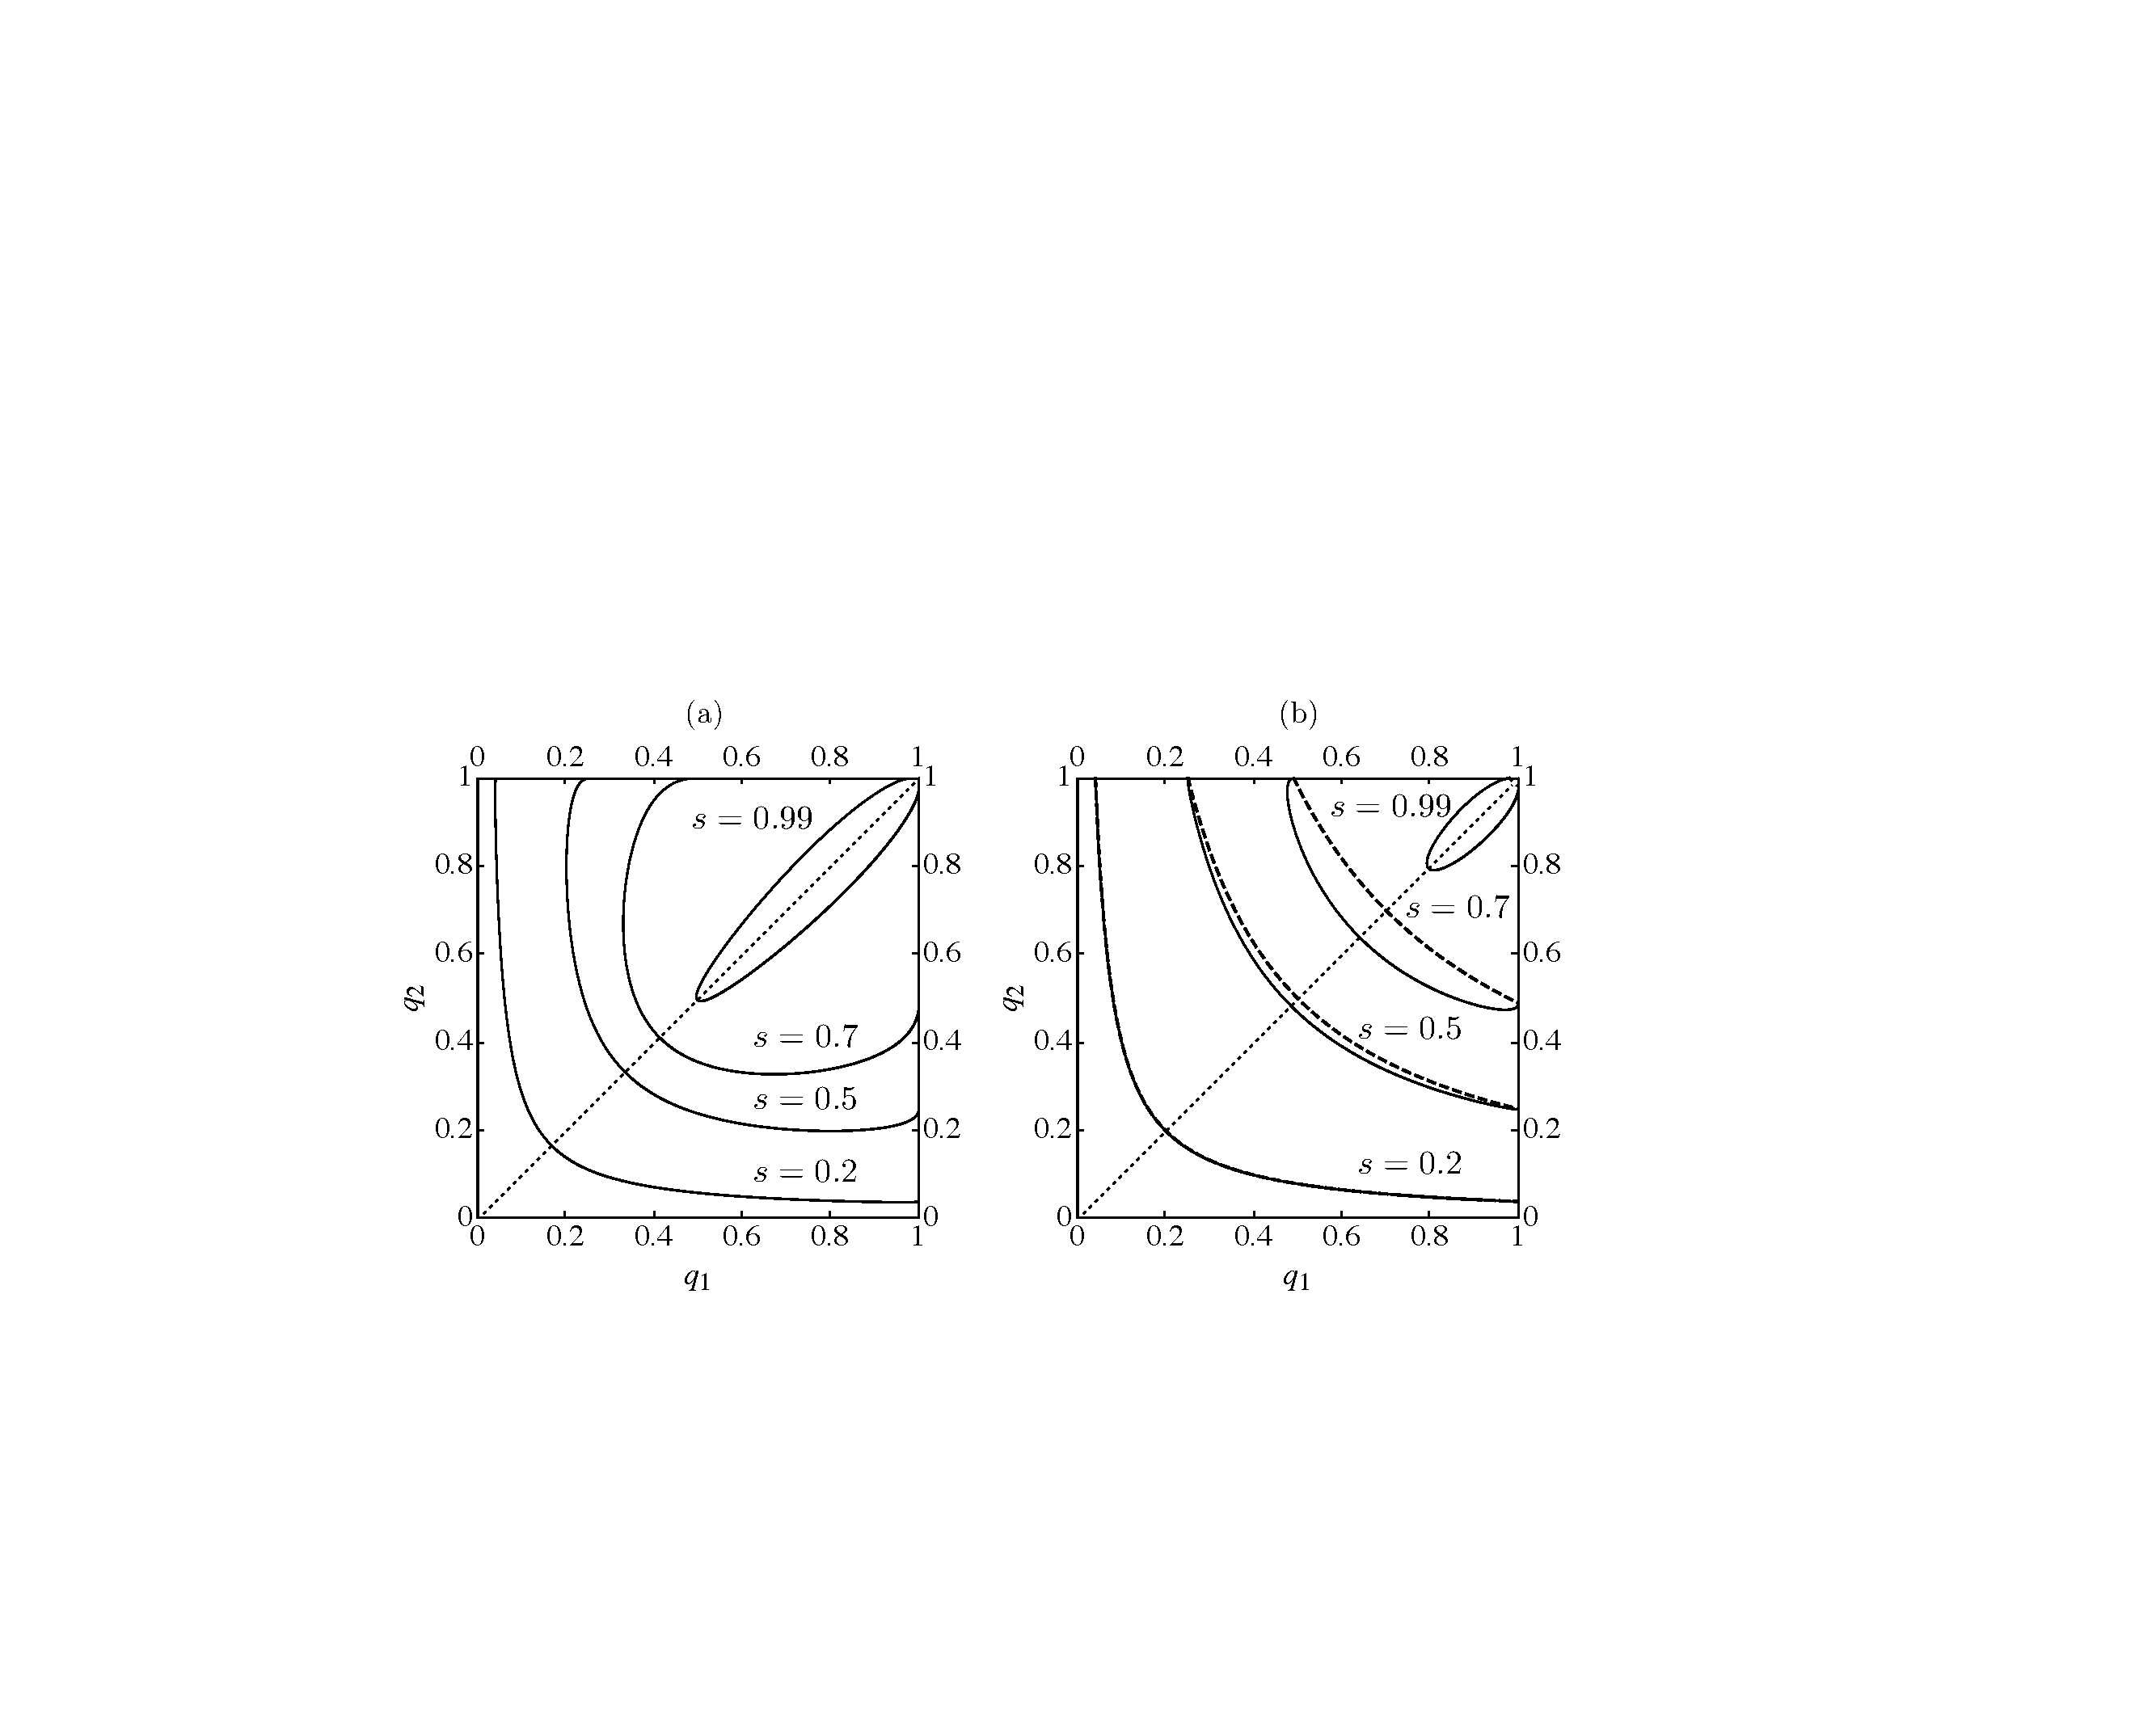
\includegraphics[width=26.5em]{Fig_2NC.pdf}\\
\end{array}%
$%
\caption{Unitarity curves for different values of the overlap~$s$ and for (a) $m=1$, $n=2$ and (b) $m=1$, $n=5$. The curves are symmetric under mirror reflexion along the  (dashed) straight line $q_1=q_2$, i.e., under the transformation~$q_1\leftrightarrow q_2$.}
\label{fig:2}
\end{figure}
%

Now we can come back to the minimization of the average failure probability $Q$. Despite the apparent simplicity of the problem finding the minimum $Q$ as an explicit function of $\eta_1$ or $\eta_2$ involves solving a sixth degree equation. No general method for solving such equations exists, so  we will derive the curve $(\eta_1,Q_{\rm min})$ in parametric form. This, along with a more detailed description of the unitary curve~(\ref{unit cond}), provides a complete account of two state dependent cloning.

Without any loss of generality we may assume that~$\eta_1\le\eta_2$, or equivalently,  that~$0\le\eta_1\le 1/2$. Then, the slope of the normal vector to the straight line~$Q=\eta_1 q_1+\eta_2 q_2$ is less or equal than one and thus it can only become tangent to the lower half of the unitary curve~(\ref{unit cond}) (see Fig.~\ref{fig:2}). It is apparent from Fig.~\ref{fig:2} that the slope of this lower half increases monotonically as we move away from the line $q_1=q_2$, where it has the value~$-1$, and vanishes before we reach the line~$q_1=1$. This can be shown analytically from the parametric form of the unitary curve given in Eq.~(\ref{par trig}) or Eq.~(\ref{par sqrt}). More precisely, the values of $t$ at which the slope is $-1$ and $0$ are respectively
%
\begin{equation}
t_{-1}={1-s^{n-m}\over 1-s^n},\quad
t_0={1-s^{2(n-m)}\over 1-s^{2n}},
\label{t's}
\end{equation}
%
where we note that $t_{-1}$ is the lower value of the range of $t$ is in Eq,~(\ref{range t}). For any point whose value of $t$ in the range~$[t_{-1},t_0]$ there is a line $Q=\eta_1 q_1+\eta_2 q_2$ that is tangent to it, starting with $\eta_1=\eta_2=1/2$ for $t=t_{-1}$ up to $\eta_1=0$, $\eta_2=1$ for $t=t_0$. This observation enables us to derive the desired parametric expression for the optimality curve~$(\eta_1,Q_{\rm min})$ as follows. At a given $t$ in the range above a necessary condition for tangency is \mbox{$\eta_1 q'_1+\eta_2 q'_2=0$}, where $q'_i=d q_i/d t$. In this equation we can solve for $\eta_1$ (or $\eta_2$) using that $\eta_1+\eta_2=1$. By substituting $q_1$ and~$q_2$ in $Q_{\rm min}=\eta_1 q_1+\eta_2 q_2$ with~(\ref{par trig}) or~(\ref{par sqrt}) we enforce contact with the unitarity curve. The final result can be cast as:
%
\begin{equation}
\eta_1={q'_2\over q'_2-q'_1},\;\; Q_{\rm min}={q'_2 q_1-q'_1 q_2\over q'_2-q'_1},\;\; t_{-1}\le t\le t_0,
\end{equation}
%
where $t_{-1}$, $t_0$ and $q_i$ are given in Eqs.~(\ref{t's}), (\ref{par trig}) and~(\ref{par sqrt}). The expressions for the derivatives $q'_i$ are most easily derived from the trigonometric form~(\ref{par trig}) to be
%
\begin{equation}
q'_i={\sqrt{q_i(1-q_i)}\over s^{n-m}}\left\{{1+s^n\over\sqrt{1-x^2}}-(-1)^i{1-s^n\over\sqrt{1-y^2}}\right\}.
\end{equation}
%

Fig.~\ref{fig:3} shows plots of the curves $(\eta_1,Q_{\rm min})$ for $m=1$ input copies and  (a) $n=2$ or (b) $n=5$ clones, as in the previous figure. We see that $Q_{\rm min}$ is an increasing function of $\eta_1$ in the given range $[0,1/2]$. The values of~$Q_{\rm min}$ at the end points of this range follow by substituting $t_{0}$ and $t_{-1}$, Eq.~(\ref{t's}), into Eq.~(\ref{par sqrt}). They are given by
%
\begin{equation}
Q_{0}=q_2(t_0)={s^{2m}-s^{2n}\over 1-s^{2n}},\quad
Q_{-1}={s^m-s^n\over 1-s^n},
\end{equation}
%
where $Q_{\rm min}=Q_{-1}$ holds for equal priors.

\begin{figure}[h]
\centering
$%
\begin{array}{c}
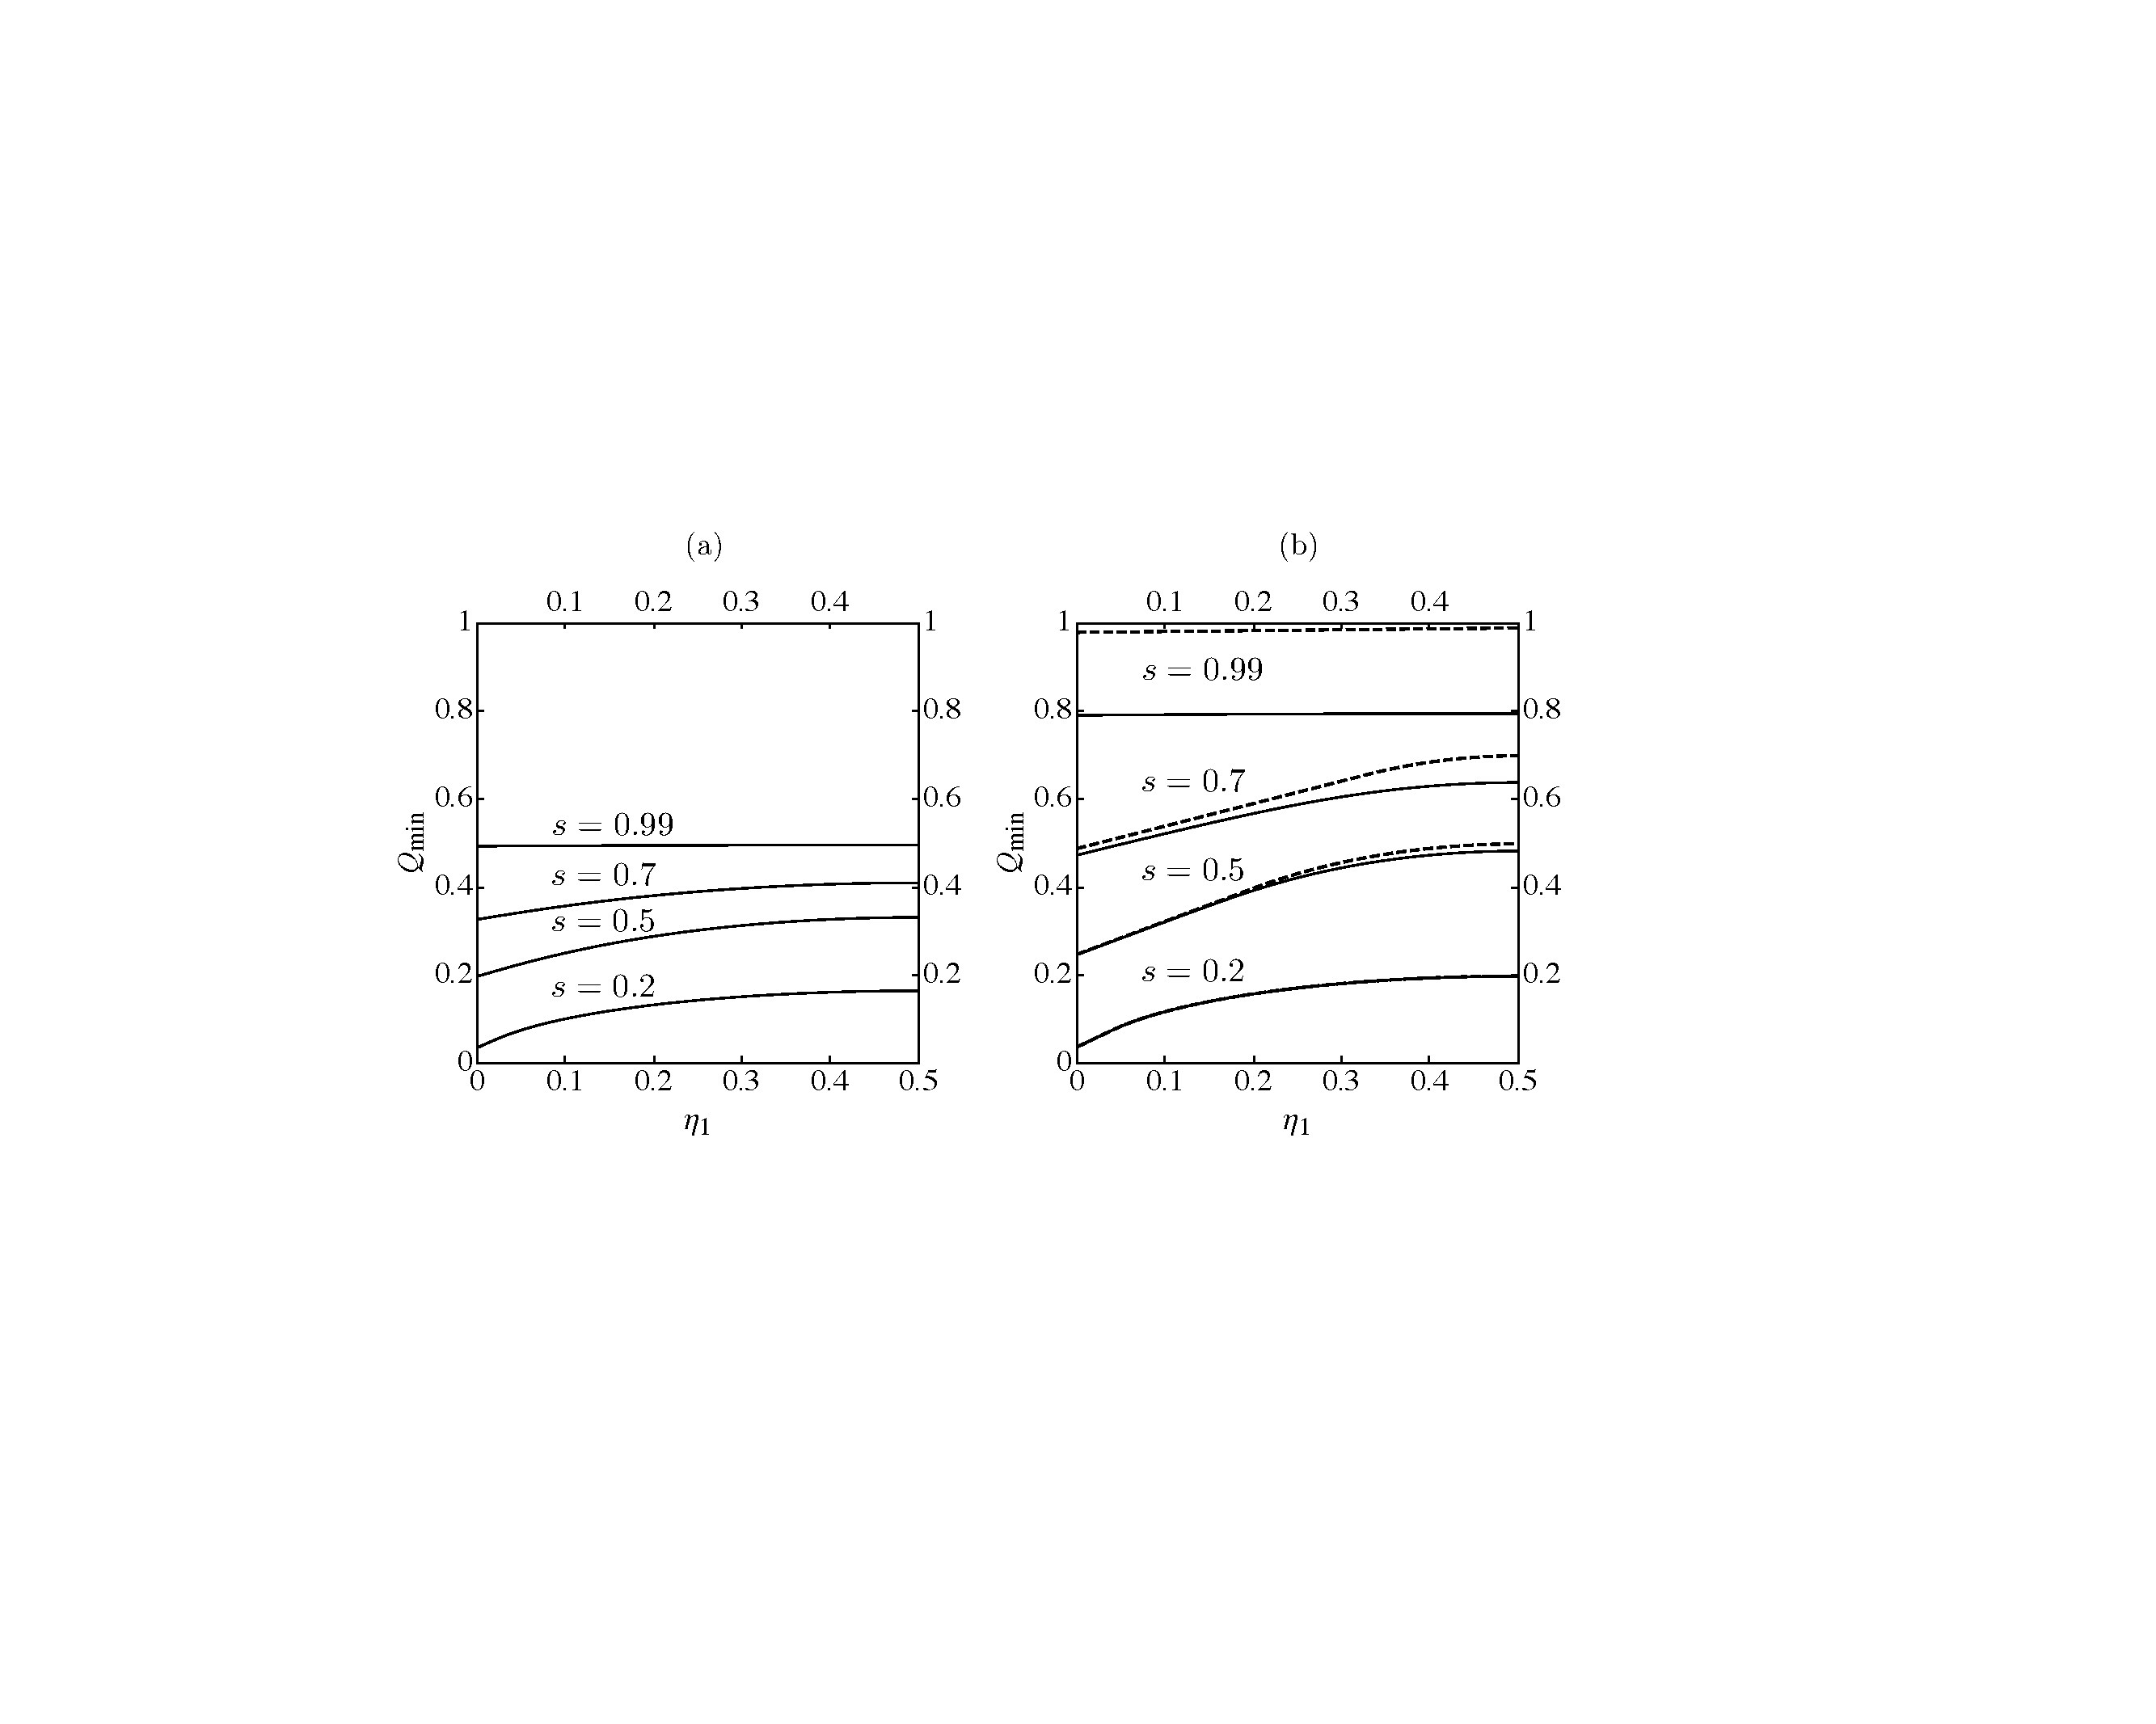
\includegraphics[width=26.7em]{Fig_3NC.pdf}\\
\end{array}%
$%
\caption{$Q_{\rm min}$ vs. $\eta_1$ for the same values of $m$, $n$ and $s$ used in the previous figure.}
\label{fig:3}
\end{figure}

Before summarizing, we would like to go back to the relationship to state discrimination.  It was mentioned above that  the limit $n \rightarrow \infty$ leads to the probabilities associated with optimal unambiguous discrimination of the pure states $|\psi_1^m\rangle$ and $|\psi_2^m\rangle$.  This curve is identical to the $\alpha = 0$ curve in Fig. 1.  UD measurements are sometimes projective, and other times POVM's, depending on the given conditions, but there is no apparent distinction in these graphs.  Closer inspection shows us that the curves in Fig. 2 all have slopes in the interval $(0,\infty)$, while the UD hyperbola given by $q_1 q_2 - s^2 = 0$ may not.   Specifically, at the limiting point $(q_1,q_2) = (1,s^2)$ the normal vector is $(s^2,1)$.  If $\eta_2/\eta_1 > 1/s^2$, the optimal line $Q = \eta_1 q_1 + \eta_2 q_2$ cannot be tangent to the unitary curve, as that tangency would be beyond the permissible domain.  Therefore it pivots on the point $(1,s^2)$ as $\eta_2/\eta_1$ increases, implying $Q = \eta_1 + \eta_2 s^2$.  This is the well-known result of the projective measurement domain in unambiguous state discrimination.  While this feature exists for the limiting case $N \rightarrow \infty$, it does not appear for any finite $N$ number of clones, because the line representing the optimal failure rate can always be tangent to the unitary curve for any values of initial prior probabilities.  This means that the deterministic cloning process is inherently smooth.

Going beyond pure states in perfect probabilistic cloning schemes is significantly more difficult, and there exist general results for other types of states  \cite{Fiurasek1,}. Experiments have been suggested \cite{ Fiurasek1} and implemented \cite{Muller} for cloning quantum states.

As mentioned earlier, there is a deep relationship between cloning and state discrimination, where the asymptotic behavior of cloning strategies has been shown to reproduce known measurement results \cite{ Chefles1,Bae}. More information may be found in a review \cite{review1}
  
Moreover, the probabilistic nature of states offers fertile ground for research on physics' connections to classical probability and statistics such as quantum statistical inference \cite{Mallery,Nielsen}. 

\begin{thebibliography}{99}

\bibitem{Pomarico}E. Pomarico et all, Optics and Spectroscopy \textbf{111}, Issue 4, 510-519 (2011)


\bibitem{Gisin} N. Gisin, B. Huttner Physics Letters A, \textbf{ 228}, Issues 1–2, 13–21 (1997)

\bibitem{Mallery} James D. Malley and John Hornstein, Statistical Science \textbf{8}  No. 4,  433-457 (1993)

\bibitem{Nielsen} Ole E. Barndorff-Nielsen, Richard D. Gill andPeter E. Jupp, Journal of the Royal Statistical Society: Series B 
\textbf{65}, 775–804 (2003)

\bibitem{Gisin1}N. Gisin and S. Massar, Phys. Rev. Lett. \textbf{79}, 2153 (1997)

\bibitem{Buzek} Vladimír Bužek and Mark Hillery, Phys. Rev. Lett. \textbf{81}, 5003 (1998)

\bibitem{Brub}Dagmar Bruß, Phys. Rev. A 57, 2368  { 1998}


\bibitem{Chefles1} Anthony Chefles and Stephen M. Barnett, Phys. Rev. A \textbf{60}, 136  (1999)

\bibitem{Fiurasek} J. Fiurášek, S. Iblisdir, S. Massar, and N. J. Cerf, Phys. Rev. A \textbf{65}, 040302(R) (2002)


\bibitem{DuanGuo} Lu-Ming Duan and Guang-Can Guo, Phys. Rev. Lett. \textbf{80}, 4999  (1998)


\bibitem{Fiurasek1} Jaromír Fiurášek,  Phys. Rev. A \textbf{70}, 032308 (2004)


\bibitem{Muller} Christian R. Müller, et. all, Phys. Rev. A \textbf{86}, 010305(R) (2012)

\bibitem{Bae} Joonwoo Bae and Antonio Acin, Phys. Rev. Lett. \textbf{97}, 030402 (2006)

\bibitem{review1} Valerio Scarani, Sofyan Iblisdir, and Nicolas Gisin, Reviews of Modern Physics \textbf{77}, 1225-1256 (2005)













Lu-Ming Duan and Guang-Can Guo
\end{thebibliography}     
\end{document}
